%
% ****
\chapter{Grundlagen der neuronalen Netze}
\label{chap:neuro}
% ****
%
	Dieses Kapitel dient als Einführung in meine Arbeit und zeigt auf, wie im Laufe der Zeit das Konstrukt der neuronalen Netze erforscht und zu Nutze gemacht wurde. Darüber hinaus wird die Notwendigkeit einer Alternative zum klassischen Modell der Rechenmaschine aufgezeigt und genauer beleuchtet. Um die Performance dieser klassischen Automaten bzw. Rechenmaschinen zu testen, werden einige Berechenbarkeitsmodelle vorgestellt. Die einzigartige Umsetzung in Netzwerken neuronaler Nervenzellen ermöglicht es uns, hochkomplexe Aufgaben selbst bei niedrigen Taktfrequenzen durch hohe Parallelität zu bewältigen. Im weiteren Verlauf wird auch auf die Notation und Beschaffenheit neuronaler Netze eingegangen. \\
	Dieser Abschnitt der Bachelorarbeit lehnt sich besonders an die ersten Kapitel der folgenden Bücher an: \textit{R.Rojas - Theorie der neuronalen Netze} \cite{TheorieNeuro} und \textit{Gerstner et al. - Neuronal Dynamics} \cite{NeuronalDynamics}. Weitere Fachartikel werden im Laufe des Kapitels genannt.
% ***
\section{Grundlegende Berechenbarkeitsmodelle}
\label{sec:neuro_models}
% ***
	Im Bereich der Berechenbarkeitstheorie (oder auch Rekursionstheorie) werden Probleme auf die Realisierbarkeit durch ein mathematisches Modell einer Maschine bzw. einem Algorithmus untersucht und kategorisiert. Diese Theorie entwickelte sich aus der mathematischen Logik und der theoretischen Informatik. Neuronale Netze bieten hier eine alternative Formulierung der Berechenbarkeit neben den bereits etablierten Modellen an. Es existieren die folgenden fünf Berechenbarkeitsmodelle, welche durch einen mathematischen oder physikalischen Ansatz versuchen, ein gegebenes Problem zu lösen:
	\begin{itemize}
		\item Das mathematische Modell
			\subitem Die Frage nach der Berechenbarkeit wird in der Mathematik durch die zur Verfügung stehenden Mittel dargestellt. So sind primitive Funktionen und Kompositionsregeln offensichtlich zu berechnen, komplexe Funktionen, welche sich nicht durch primitive Probleme darstellen lassen, jedoch nicht. Durch die \textit{Church-Turing-These}\footnote{Alonzo Church \& Alan Turing, 1936} wurden die berechenbaren Funktionen wie folgt abgegrenzt: "'Die berechenbaren Funktionen sind die allgemein rekursiven Funktionen."'
		\item Das logisch-operationelle Modell (Turing Maschine)
			\subitem Durch die Turing Maschine \footnote{Alan Turing, 1936} konnte neben der mathematischen Herangehensweise an Berechenbarkeitsprobleme eine mechanische Methode eingesetzt werden. Die Turing Maschine nutzte ein langes Speicherband, welches nach gewissen Regeln schrittweise Manipuliert wurde. So konnte sie sich in einer bestimmten Anzahl von Zuständen befinden und nach entsprechenden Regeln verfahren.
		\item Das Computer-Modell
			\subitem Kurz nach dem bahnbrechenden Erfolg von Turing und Church wurden viele Konzepte für elektrische Rechenmaschinen entworfen. Konrad Zuse entwickelte in Berlin ab 1938 Rechenautomaten, welche jedoch nicht in der Lage waren, alle allgemein rekursiven Funktionen zu lösen. Der Mark I, welcher um 1948 an der Manchester Universität gebaut wurde war der erste Computer, welcher alle rekursiven Funktionen lösen konnte. Er verfügte über die damals etablierte Von-Neumann-Architektur\footnote{John von Neumann, 1945} und wurde von Frederic Calland Williams erbaut.
		\item Das Modell der Zellautomaten
			\subitem John von Neumann arbeitete darüber hinaus auch an dem Modell der Zellautomaten, welches eine hoch-parallele Umgebung bot. Die Synchronisation und Kommunikation zwischen den Zellen stellt sich jedoch als herausfordernde Problemstellung heraus, welche nur durch bestimmte Algorithmen gelöst werden kann. Eine solche Umgebung liefert, wenn richtig umgesetzt, eine enorme Rechenleistung dank Multiprozessorarchitektur selbst bei geringen Taktfrequenzen.
		\item Das biologische Modell (neuronale Netze)
			\subitem Neuronale Netze heben sich nun von den vorher beschriebenen Methoden ab. Sie sind nicht sequentiell aufgebaut und können, anders als Zellautomaten, eine hierarchische Schichtenstruktur besitzen. Die Übertragung von Informationen ist daher nicht nur zum Zellnachbarn,  sondern im ganzen Netzwerk möglich. Jedoch wird im neuronalen Netz nicht (wie in der Rechenmaschine üblich) ein Programm gespeichert, sondern es muss durch die s.g. Netzparameter erlernt werden. Dieser Ansatz wurde früher durch mangelnde Rechenleistung der konventionellen Computer nicht weiter verfolgt. Jedoch erfahren wir heute immer mehr den Aufwind neuester Lernalgorithmen und Frameworks, die das Arbeiten im Bereich Deep Learning, Artificial Intelligence und adaptives Handeln unheimlich unterstützen und beschleunigen. Weitergehend ist man heute in der Lage, auf dem Gebiet der Biologie Nervensysteme zu analysieren und von Millionen Jahren der Evolution zu profitieren. So können verschiedene neuronale Netze genauestens beschrieben und simuliert werden.
	\end{itemize}
% ***
\section{Die biologische Nervenzelle}
\label{sec:neuro_nervenzelle}
% ***
	Zellen, wie sie in jeder bekannten Lebensform auftreten, sind weitestgehend erforscht und gut verstanden. Wie alle Zellen im Körper bestehen Sie (stark vereinfacht) aus einer Zellmembran, einem Zellskelett und einem Zellkern, welcher die chromosomale DNA und somit die Mehrzahl der Gene enthält. Sie treten im menschlichen Körper in verschiedenen Größen und mit unterschiedlichen Fähigkeiten auf. Neuronale Nervenzellen wurden über die Evolution dahingehend ausgeprägt, dass sie Informationen Empfangen, verarbeiten und entsenden können. Wie in Abb. \ref{fig:neuron} zu sehen, besteht eine Nervenzelle aus drei Bestandteilen: \textit{Dendrit, Soma und Axom}.
	\begin{figure}[!h] %[!t] ...
		\centering
		\def\svgwidth{12cm}
		\input{figures/chap_neuron/neuron_is.pdf_tex}
		%\includegraphics[width=4cm]{figures/neuron.svg}
		\caption{Schematische Darstellung einer Nervenzelle bestehend aus Dendrit, Soma und Axon.}
		\label{fig:neuron}
	\end{figure}
	\begin{itemize}
		\item Dendrit:
			\subitem Der Dendrit (altgr. 'Baum') dient der Reizaufnahme in der Nervenzelle. Gelangen durch andere Nervenzellen Spannungsspitzen durch vorhandene Synapsen an den Dendrit, leitet dieser die Signale an die Soma weiter.
		\item Soma:
			\subitem Die Zellsoma bezeichnet den allg. Körper der Zelle. Es umfasst den plasmatischen Bereich um den Zellkern, ohne die Zellfortsätze wie Dendriten und Axon. Hier findet der Hauptteil des Stoffwechsels statt, alle ankommenden Signale aus den Dendriten werden integrierend verarbeitet und eine Änderung des Membranpotentials findet statt. Empfangene Signale können erregend oder hemmend auf den Summationsprozess wirken (Siehe Kap. x - LIF Modell). Überschreitet das Membranpotential einen gewissen Threshold, so reagiert die Soma und erzeugt einen Spannungsstoß, welcher an das Axon gegeben wird.
		\item Axon:
			\subitem Das Axon (altgr. 'Achse') ist ein Nervenzellfortsatz, welcher für die Weiterleitung der Signale von der Soma an die Synapsen und damit an andere Nervenzellen verantwortlich ist.
	\end{itemize}
	Verbunden sind Nervenzellen durch s.g. Synapsen, welche den Informationsfluss gewährleisten. Der Informationsfluss geschieht in Synapsen größtenteils chemisch. Bei einem ankommenden Aktionspotential werden Neurotransmitter aus der Zelle ausgeschüttet, welche für einen Ionentransport verantwortlich sind. Nach Übertragung der chemischen Stoffe über den Synapsenspalt werden diese wieder in ein elektrisches Potential umgewandelt. Diese Synapsen treten zwischen benachbarten Nervenzellen bzw. auf kurzer Distanz auf. Elektrische Synapsen hingegen sind noch weitestgehend unerforscht. Sie dienen als Kontaktstellen und ermöglichen eine Übertragung von Ionen und kleineren Molekülen von einer Zelle zur anderen. Die Signalübertragung entfernter Nervenzellen wird somit synchronisiert. Man bezeichnet sie auch als '"Gap-Junctions'". Im weiteren Verlauf dieser Arbeit werden Synapsen nach Abb. \ref{fig:synapse} dargestellt.\\
	\begin{figure}[!h] %[!t] ...
		\centering
		\def\svgwidth{12cm}
		\input{figures/chap_neuron/synapse_is.pdf_tex}
		\caption{Darstellung von verschiedenen Synapsen-Typen.}
		\label{fig:synapse}
	\end{figure}\\
	Bei chemischen Synapsen ist zwischen exzitatorischen und inhibitorischen Synapsen zu unterscheiden. Erstgenannte agieren als erregende Synapsen und übertragen das Aktionspotential mit positivem Vorzeichen an die postsynaptische Nervenzelle. Inhibitorische Synapsen sind hingegen hemmender Natur und führen das Potential mit einem negativen Vorzeichen, sodass es entsprechend negativ gewichtet in den Integrationsprozess der postsynaptischen Nervenzelle eingeht.
% ***
\section{Das biologische neuronale Netz}
\label{sec:neuro_netz}
% ***
	Funktionsweisen neuronaler Netze sind bereits gut erforscht und modelliert worden. Besonders das Nervensystem des Wurms \textit{C. Elegans} \cite{CElegans} ist das bisher am besten verstandene Konstrukt in diesem Bereich der neuronalen Forschung. In dieser Arbeit wird insbesondere auf den s.g. \textit{Touch-Withdrawal-Circuit} eingegangen und versucht, eine Implementierung zu schaffen, welche ein dynamisches System erfolgreich regeln kann.\\
	Ausgangspunkt ist das bereits von Lechner et al. \cite{WormLevelRL} grafisch dargestellte neuronale Netz des C. Elegans, welches den Berührungs-Reflex des Wurms modelliert.
	\begin{figure}[!h] %[!t] ...
		\centering
		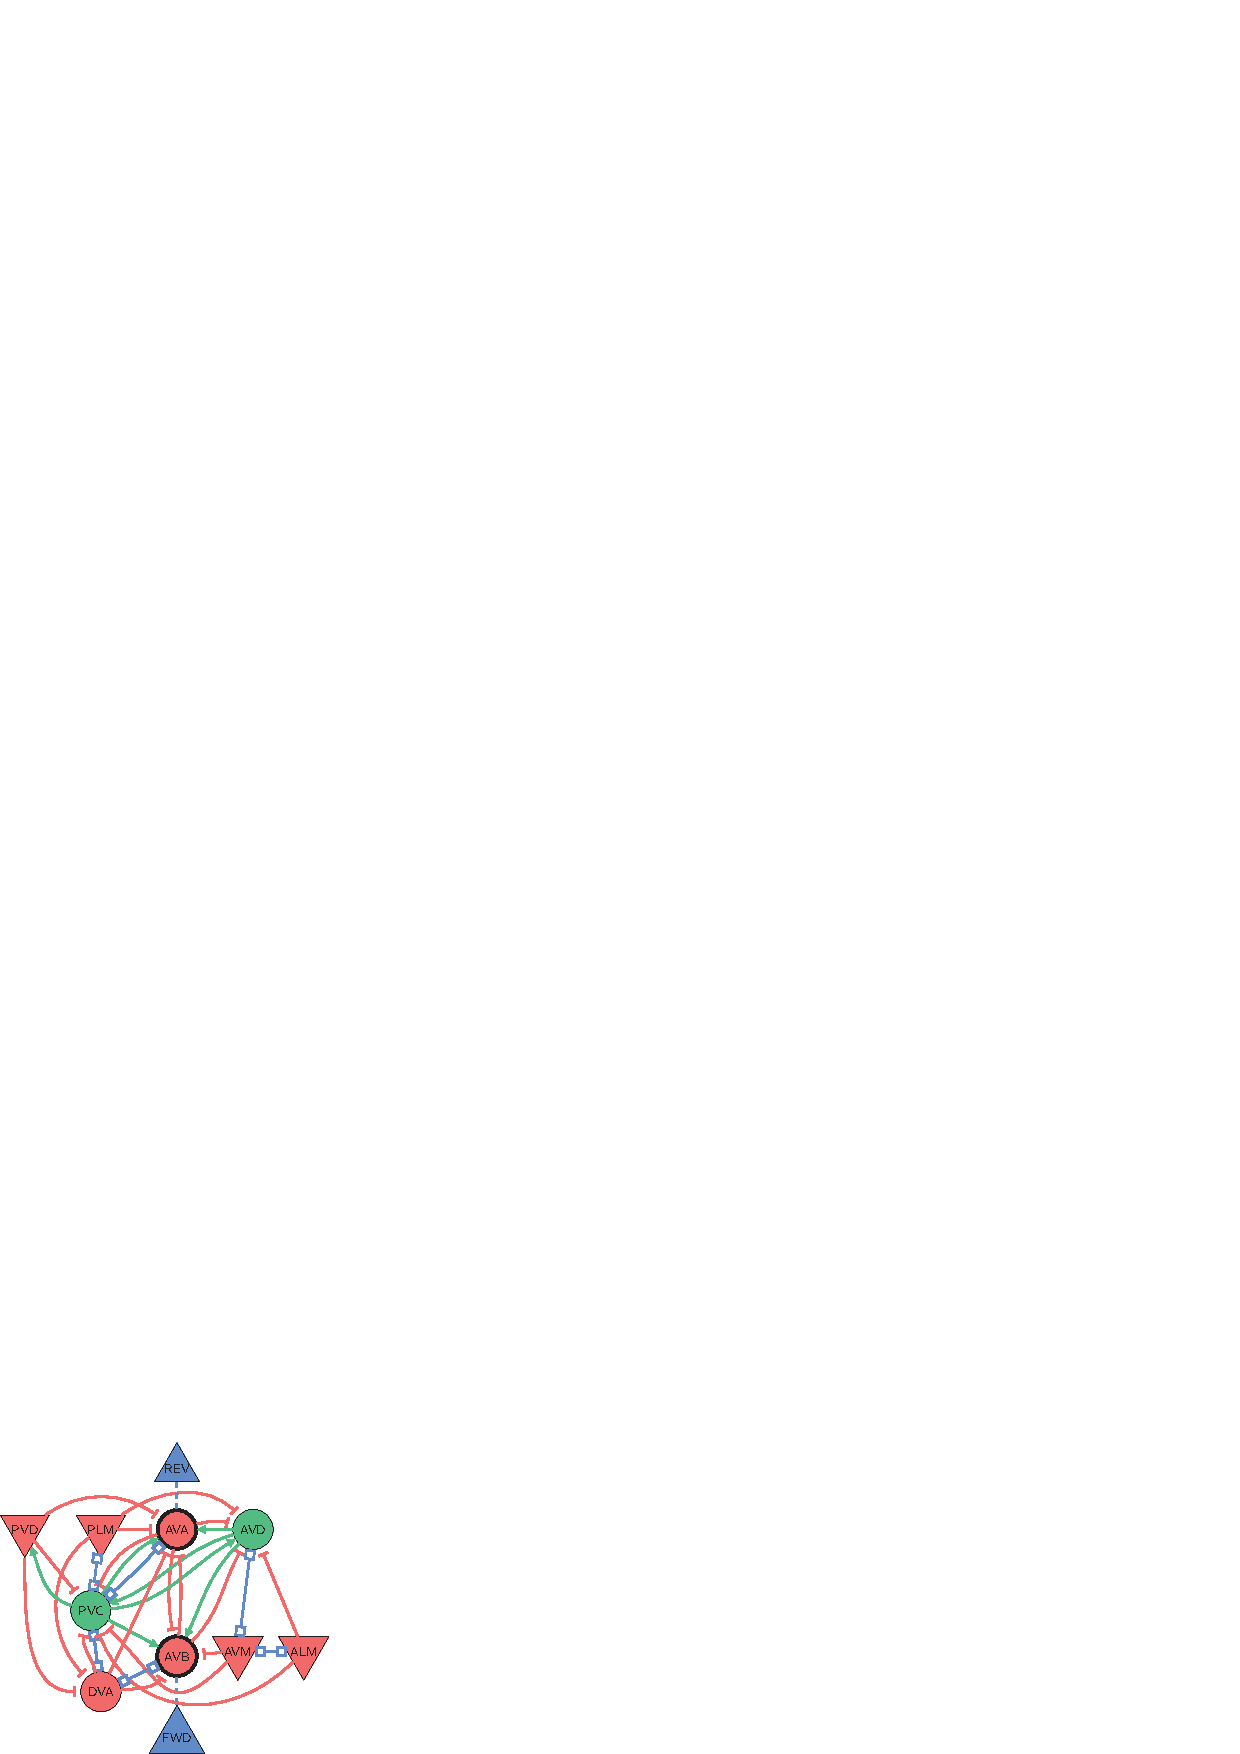
\includegraphics[width=6cm]{figures/chap_neuron/Orig_TW_Circuit.pdf}
		\caption{TW-Neuronal-Circuit nach Lechner et al. \cite{WormLevelRL}}
		\label{fig:01_TW-Circuit}
	\end{figure}
	Wird der Wurm einem äußeren Stimulus - sprich einer Berührung - ausgesetzt, so schnellt er zurück. Anhand des Schaubilds lässt sich nachvollziehen, was in dem Fall einer Berührung in dem neuronalen Netz geschieht:\\
	Die Sensor-Neuronen PVD, PLM, AVM und ALM stellen Rezeptoren dar und reagieren auf Berührung. Sie transduzieren in diesem Fall die Berührung in eine neuronal vergleichbare Form als Aktionspotential und übermitteln diese Information durch die gegebenen Synapsen inhibitorisch oder exzitatorisch an die verbundenen internen Nervenzellen. Dieses Potential beträgt je nach gegebener Intensität der Berührung zwischen $-70mV$ (Ruhespannung - keine Berührung) und $-20mV$ (Spike-Potential - maximale Berührungsintensität) und bildet den Aktionsraum $A\in[-70mV, -20mV]$. Die genannten Sensor-Neuronen lassen sich so beliebig einsetzen und stellen bspw. im Experiment des inversen Pendels positive und negative Observationsgrößen dar. Eine beispielhafte Belegung wäre die folgende:
	\begin{center}
	\begin{tabular}{c@{\hskip 0.5cm}c@{\hskip 0.5cm}c@{\hskip 0.5cm}c}    \toprule
		\setlength{\tabcolsep}{50pt}
		\renewcommand{\arraystretch}{1.5}
		\emph{Umgebungsvariable} & \emph{Typ}  & \emph{Posivite Sensor-Neurone} & \emph{Negative Sensor-Neurone} \\\midrule
		$\varphi$ 				 & Observation & PLM							& AVM							 \\ 
		$\dot{\varphi}$		 	 & Observation & ALM							& PVD							 \\
		$a$						 & Action	   & FWD							& REV							 \\\bottomrule
		\hline
	\end{tabular}
	\end{center}
	Im weiteren Verlauf der Bachelorarbeit werden zudem Vor- und Nachteile aufgezeigt, die genannten Sensor-Neuronen mit anderen Observationsgrößen zu belegen.\\
	Interneuronen, wie PVC, AVD, DVA, AVA und AVB sind direkt mit Sensor-Neuronen sowie untereinander durch Synapsen und Gap-Junctions verbunden. In jeder internen Nervenzelle findet ein Integrationsprozess der jeweiligen anliegenden Ströme aus Stimulus ($I_{Stimuli}$), anderen chemischen Synapsen ($I_{Syn}$) und Gap-Junctions ($I_{Gap}$) statt. Durch das Leaky Integrate and Fire - Modell kann das Membranpotential durch anliegende Ströme zum nächstgelegenen Zeitpunkt bestimmt und ein mögliches Feuer-Event vorhergesagt werden. Eine Nervenzelle feuert ein Signal, wenn das Membranpotential einen Treshold $\theta = -20mV$ erreicht hat. Neurotransmitter werden freigelassen und ein Informationsfluss findet statt.\\
	Um nun den Reflex des Wurms C. Elegans umzusetzen benötigt es noch zwei \textit{Motor-Neuronen}. Diese sind dafür zuständig, ein Befehl in Form eines Feuer-Signals an gewisse Muskelgruppen zu übersetzen, damit diese bewegt werden. In dem behandelten Experiment bedient die Inter-Neurone AVA die Motor-Neurone REV, welche für eine Rückwärtsbewegung steht, analog die Inter-Neurone AVB die Motor-Neurone FWD, welche eine Vorwärtsbewegung initiiert.\\
	Dieser Kreislauf bildet nun ein in sich geschlossenes System mit vier Eingängen und zwei Ausgängen (man achte auf das Mapping mit positiven und negativen Werten) und bildet ein lernfähiges neuronales Netz.
% ***
\section{Das symmetrische neuronale Netz}
\label{sec:my_net}
% ***
	Wie in \cite{Wicks1996} bereits thematisiert, wird in Abb. \ref{fig:01_TW-Circuit} lediglich eine Hälfte des symmetrischen neuronalen Netzes des Wurms C. Elegans beschrieben. Wie im menschlichen Gehirn besteht das Netzwerk aus zwei Hälften, welche zusammenwirken und bei gegebenen Sensor-Input eine Aktion wählen. Eine erweiterte Analyse des Netzwerks besonders mit den berechneten Gewichten der einzelnen Synapsen ergibt, dass das gegebene Netz von Lechner et al. \ref{fig:01_TW-Circuit} unsymmetrisch scheint. Die Nervenzelle \textit{DVA}, welche als Synchronisationszelle zwischen beiden Netzwerkhälften dienen soll, taucht im gegebenen Netz als unsymmetrische Komponente auf und scheint gewisse Sensor-Inputs ungleichmäßig zu gewichten. Im Zuge dessen wird ein neues, symmetrisches neuronales Netz entwickelt, welches zum einen symmetrischer Natur ist, zum anderen manche Synapsen und Gap-Junctions misst, da diese nicht zielführend für das gegebene Problem erschienen. Spätere Simulationen bestätigten diese Annahmen, indem durch Gewichtung der Synapsen und Gap-Junctions manche Verbindungen ein verschwindend geringes Gewicht erhielten.
	\begin{figure}[!h] %[!t] ...
		\centering
		\includegraphics[width=10cm]{figures/chap_neuron/Neural_Net_v3_plain.pdf}
		\caption{Symmetrisches neuronales Netz des TW-Circuits}
		\label{fig:nn_new}
	\end{figure}\\
	Das in Abb. \ref{fig:nn_new} dargestellte, symmetrische neuronale Netz des TW-Circuit wird für alle weiteren Analysen und Simulationsläufe verwendet. Die genaue Umsetzung wird in Kapitel \ref{chap:imp} weiter erläutert.
	

%%% Local Variables: 
%%% mode: latex
%%% TeX-master: "main"
%%% End: 
